
\chapter{Manual}
\label{cha:manual}

The project code and documentation is hosted on the \texttt{masci-tools}
repository \cite{masci-tools} under the branch
\href{https://github.com/JuDFTteam/masci-tools/tree/studentproject18ws}{\texttt{studentproject18ws}}.
All of the project code resides in the folders \texttt{binder} (for the web
frontend demo) and \texttt{studentproject18w} (all code and documentation). The
\texttt{README.md} in the latter folder serves as the manual. Therefore, the
remaining part of this chapter is a \TeX{}-ified version of that
\texttt{README.md}, commit
\href{https://github.com/JuDFTteam/masci-tools/tree/b671271835aaaf36c9b7f1f227e81f1398251d1a/studentproject18w}{\texttt{b671271835aaaf36c9b7f1f227e81f1398251d1a}}.

\vspace{3em}
\hdashrule{\textwidth}{2pt}{2pt}
%% BEGIN TEXIFIED README ========================================
%% 
%% Command to TeXify README.md from masci-tools/studentproject18ws:
%% pandoc -s README.md -o README.tex
%% 
%% Manual changes needed after TeXification:
%% - update commit SHA-1 above!
%% - remove badges on top (binder badge, ...)
%% - 'try it out here on': convert to ordinary link without binder badge image
%% - figure -> figure*
%% - texttt{long} -> path{long} (enables linebreak)
%% - '\textgreater{}' -> '>'
%% - replace code sections 'Tok' with lstlisting:
%% \begin{lstlisting}[language=python, style=code]
%% \end{lstlisting}
%% 

\href{https://www.aices.rwth-aachen.de/en/academics/masters-program-simulation-sciences}{SiScLab
2018} Student Project \textbf{Analysis Tool for Materials
  Design}. Written in Python3.

Authors: \href{https://github.com/Irratzo}{Johannes Wasmer},
\href{https://github.com/ChristianPartmann}{Christian Partmann}, and
\href{https://github.com/PraneethKatta}{Praneeth Katta}.

\section{Overview}\label{overview}

This subfolder \texttt{studentproject18ws} is currently a largely
independent side-project accompanying the main module
\texttt{masci-tools}. It was created in a student project at \href{http://www.fz-juelich.de/pgi/pgi-1/EN/Home/home_node.html}{FZJ PGI-1}, and consists
of three submodules:

\begin{itemize}
    \tightlist
\item
    preprocessor: a general
    \href{https://www.hdfgroup.org/solutions/hdf5/}{HDF5} reader interface, and
    one implementation for band structure simulation output of the DFT code \href{http://www.judft.de}{Fleur}
\item visualization: a plotting interface, and one implementation for
    \href{http://www.judft.de}{Fleur} band structure and density of states (DOS)
    plots
\item
    frontends: a desktop GUI and a web dashboard (Tk and Jupyter) for
    interactive Fleur band-DOS plots.
\end{itemize}

A more thorough description and example use cases can be found in the
project \href{./doc/report.pdf}{report} and
\href{./doc/presentation.pdf}{presentation}.

\begin{figure*}
    \centering
    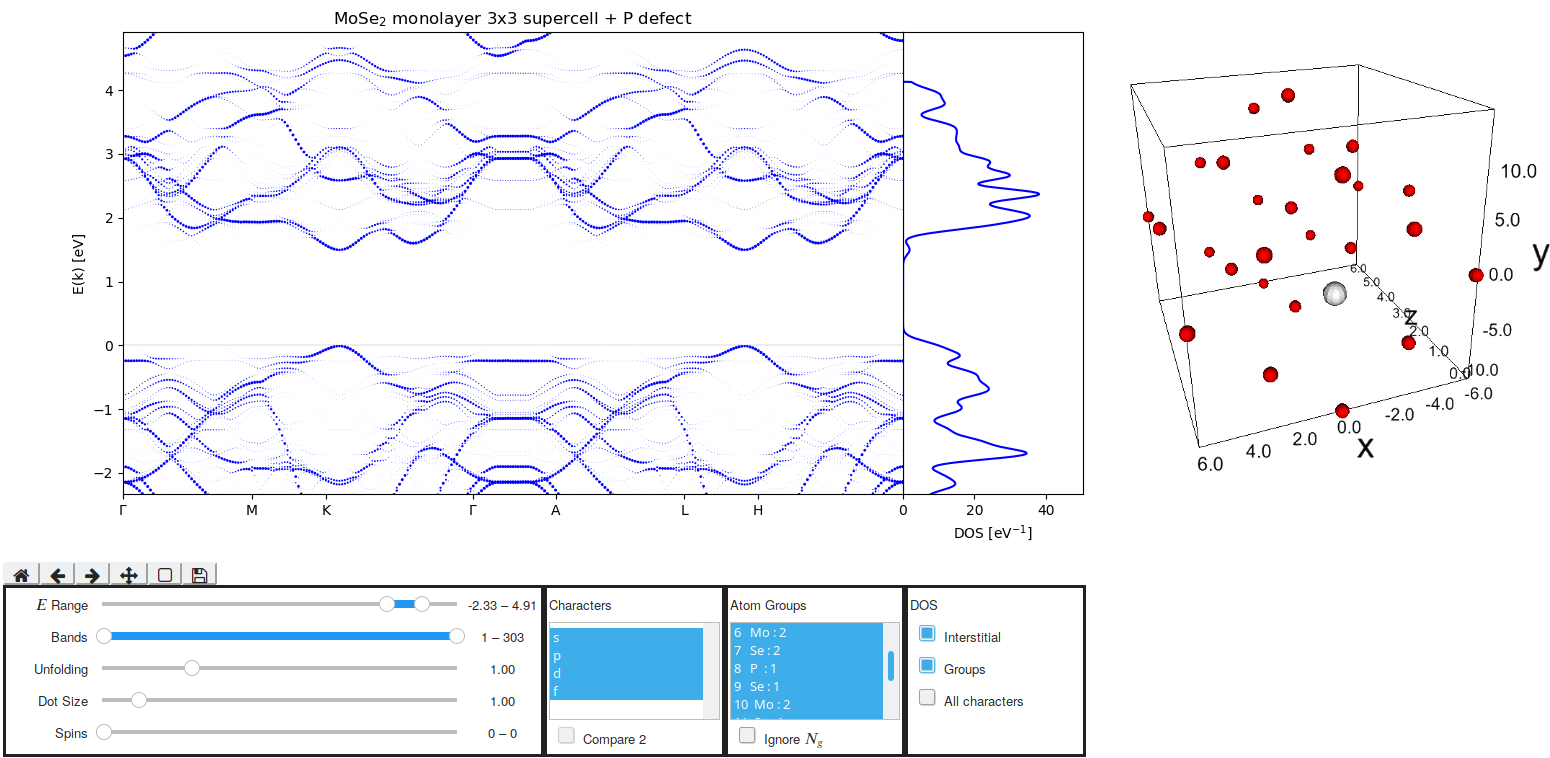
\includegraphics{./readme/web_frontend.png}
\end{figure*}

\section{For Frontend Users}\label{for-frontend-users}

\subsection{General Remarks}\label{general-remarks}

These remarks apply to all frontends.

Though the desktop and web frontend are functionally identical, there
might be small differences in how the controls are used and how they are
labeled.

\subsubsection{File Input}\label{file-input}

The frontends currently expect band structure data in the HDF output format of
\href{http://www.judft.de}{Fleur}. The DOS data is expected
to be in the CSV output format of \href{http://www.judft.de}{Fleur}, one file
per spin. If no DOS files are supplied, the frontend will just draw a band
structure plot (band plot) and omit the adjoined DOS plot. Thus, in the
following band-DOS plot stands for both kinds of plot.

\subsection{Desktop Frontend}\label{desktop-frontend}

\subsubsection{Access}\label{access}

A windows executable file (.exe) is made by packing all the required packages
into the file. Any modern PC running on windows can run the frontend without any
installation process. You don't need Python or specific packages installed.

The executable for Windows can be downloaded \href{https://rwth-aachen.sciebo.de/s/CP2dJ9M9KPDakN2}{here}. Executables for other operating systems may be requested from the developers.

\subsubsection{Usage}\label{usage}

The desktop-based GUI is easy to use. Running the .exe file will open up the
frontend with all packages loaded. The GUI consists of three tab windows. In the
first tab window, absolute paths to the input data files must be entered in this
order: HDF and (optional) DOS file for spin `0' and `1'. Tab 2 shows the
band-DOS plot, and Tab 3 the 3D atoms plot. After loading the files, the controls
must be initialized. Finally, clicking the 'Update' button produces the plots.


Controls for all three plots: 

\begin{itemize}\tightlist
\item \textbf{Update, SaveButton}: redraw the plots with the new selection / save the the plot as a PDF.
\item \textbf{Atom Groups}: redraw only for the selected symmetry groups.
\end{itemize}

Controls for the band and DOS plots:

\begin{itemize}\tightlist
\item \textbf{Ymin, Ymax}: limit the energy range.
\item \textbf{BandMin, BandMax}: limit the band range.
\item \textbf{Character}: likewise for the characters (orbitals) 'S','P','D','F'.
\item \textbf{Spin}: draw bands and DOS for one or both spins.
\end{itemize}

Controls for the band plot only:

\begin{itemize}\tightlist
\item \textbf{Marker Size}: set the marker size of the dots (eigenenergies).
\item \textbf{Exponential weight}: The unfolding exponent for supercell calculations (see \href{./doc/report.pdf}{report}). Value 0.0 means no unfolding. If the calculation is done with a unit cell, this control has no effect.
\item \textbf{Compare 2 Characters}: show the respective contribution of the two selected characters to each eigenergy using a sequential (2) colormap. Disabled if other than two characters are selected.
\item \textbf{Ignore Atom Group}: set the contribution of each group to be equal
    instead of to the number of atoms per group.
\end{itemize}

Controls for the DOS plot only:

\begin{itemize}\tightlist
\item \textbf{Select groups}: include selected atom groups in the DOS
\item \textbf{Interstitial}: include the interstitial in the DOS
\item \textbf{All characters}: include all characters in the DOS regardless of character selection. In the DOS CSV file, different input data is used (a summed column).
\end{itemize}

\subsubsection{Troubleshooting}\label{troubleshooting}

If the band plot is not visible:

\begin{itemize}
    \tightlist
\item
    Click update two to three times.
\item
    Check if the three input files (if any) are belonging to the same
    Fleur calculation and selected appropriately.
\item
    Check if at least one Atom Group, one Character, one Spin is selected.
\item
    Check if Ymin is less than Ymax and similarly BandMin is less than
    BandMax such that software is able to plot.
\end{itemize}

If the DOS plot is not visible:

\begin{itemize}
    \tightlist
\item Make sure either Select Groups or Interstitial is selected.
\end{itemize}

If the problem persists, try restarting the GUI. If that fails, please open an
issue to contact the developers.

\subsection{Web Frontend}\label{web-frontend}

\subsubsection{Access}\label{access}

The web frontend is a Jupyter Dashboard. It is in experimental state (no
fileupload yet). You can try it out
\href{https://mybinder.org/v2/gh/JuDFTteam/masci-tools/studentproject18ws?filepath=studentproject18w\%2Ffrontend\%2Fjupyter\%2Fdemo\%2Fbinder_demo.ipynb}{here
  on Binder}. You can also run it locally (see developer section). If you have an
\href{https://aiidalab.materialscloud.org/hub/login}{AiiDA Lab account}: the
dashboard is planned to be published as an app there.

\subsubsection{Usage}\label{usage-1}

Using the Dashboard should be self-explanatory to the domain user. Some
tips:

\begin{itemize}
    \tightlist
\item If the plot window is not on startup or gets stuck, reload/rerun once.
\item Plot updates are instantaneous.
\item Empty selections are impossible.
\item Only shows controls for data that is present in the input.
\item Multi-selection boxes: use ctrl or shift to select multiple items. 
\item Slider values can also be typed into the adjoining text box.
\item Try out the zoom and pan tools below the plot, they're useful.
\end{itemize}

\section{For Developers}\label{for-developers}

\subsection{Installation}\label{installation-1}

Clone this repo (branch). Then create a virtual environment for the project.

With conda (recommended): -
\href{https://www.anaconda.com/download}{Install Anaconda (3
  recommended)} - Install the environment \texttt{masci-stupro} with the
necessary and recommended dependencies:

\begin{lstlisting}[language=bash, style=code]
conda create -f environment.yml
source activate masci-stupro
\end{lstlisting}

With virtualenv (untested):

\begin{lstlisting}[language=bash, style=code]
virtualenv masci-stupro
source masci-stupro/bin/activate
pip install -r requirements_pip.txt # install requirements
\end{lstlisting}

\subsection{Programmatic use}\label{using-the-backend}

Though \texttt{masci-tools} is (planned to be) availabe via PyPI, there is
currently no plan to integrate \texttt{studentproject18ws}. If you want to use
it in your code, use it in an IDE, or append the path to your
\texttt{sys.path}:

\begin{lstlisting}[language=bash, style=code]
import sys
if path_repo not in sys.path:
    sys.path.append(path_repo)
    
# now import works
from studentproject18w.hdf.reader import Reader
# ...
\end{lstlisting}

In this example, a Fleur HDF file is preprocessed using the Recipe
\texttt{FleurBands}. The resulting output \texttt{data} with the
extracted and transformed HDF datasets and attached load methods
(Extract-Transform-Load) is then passed to a plotter, alongside some DOS
CSV files for a bandstructure plot using \texttt{matplotlib} as backend
library.

\begin{lstlisting}[language=python, style=code]
from studentproject18w.hdf.reader import Reader
from studentproject18w.hdf.recipes import Recipes
from studentproject18w.plot.matplot import BandDOSPlot
import matplotlib.pyplot as plt

data = None
reader = Reader(filepath=filepath_hdf)
with reader as h5file:
    data = reader.read(recipe=Recipes.FleurBands)
    #
    # Note:
    # Inside the with statement (context manager),
    # all data attributes that are type h5py Dataset are available
    # (on-disk access). When the statement is left, the HDF5 file 
    # gets closed and the datasets are closed.
    #
    # Use data outside the with-statement (in-memory access: all 
    # HDF5 datasets converted to numpy ndarrays):
    data.move_datasets_to_memory()

plotter = BandDOSPlot(plt, data, filepaths_dos)
(fig, ax_bands, ax_dos) = plter.setup_figure()

data_selection = some_selection_process()
plotter.plot_bandDOS(*data_selection)
plt.show()
\end{lstlisting}

\subsection{Try Out the Web Frontend
  Locally}\label{try-out-web-frontend-locally}

The demo notebook with the dashboard is
\path{studentproject18w/frontend/jupyter/demo/demo.ipynb}.

\subsubsection{If Using Jupyter
  Notebook}\label{if-using-jupyter-notebook}

On Windows, omit keyword \texttt{source}.

\begin{lstlisting}[language=bash, style=code]
source activate masci-stupro
cd mypath/masci-tools/studentproject18ws/
jupyter-notebook .
# if Home is not set to this dir, try this instead:
# /home/you/anaconda3/envs/myenv/bin/python /home/you/anaconda3/envs/myenv/bin/jupyter-notebook .
\end{lstlisting}

\subsubsection{If using Jupyter Lab}\label{if-using-jupyter-lab}

Additional installation step needed:

\begin{lstlisting}[language=bash, style=code]
source activate masci-stupro
jupyter labextension install @jupyter-widgets/jupyterlab-manager jupyter-matplotlib ipyvolume
cd mypath/masci-tools/studentproject18ws/
jupyter-lab
\end{lstlisting}

\subsection{Frontend Deployment}\label{frontend-deployment}

\subsubsection{Desktop Frontend}\label{desktop-frontend-1}

To create executables for different operating systems, use
\href{https://www.pyinstaller.org/}{PyInstaller}. The target file is
\texttt{frontend/tkinter/gui.py}.

\begin{lstlisting}[language=bash, style=code]
source activate masci-stupro
conda install -c conda-forge pyinstaller
# if not using conda: pip install pyInstaller
cd mypath/masci-tools/studentproject18ws/
pyinstaller --onefile frontend/tkinter/gui.py
\end{lstlisting}

\subsubsection{Web Frontend}\label{web-frontend-1}

The web frontend is currently a single Jupyter notebook. In order to
publish it as a usable standalone app, additional work has to be done.

\begin{itemize}
    \tightlist
\item
    Create \texttt{frontend/jupyter/Dashboard.py} and
    put code of
    \href{./frontend/jupyter/demo/demo_backend.ipynb}{demo\_backend.ipynb}
    notebook inside it. This will become the widget. Use 
    \href{https://github.com/aiidalab/aiidalab-widgets-base/blob/master/aiidalab_widgets_base/structures.py}{aiidalab-widgets-base
      > StructureUploadWidget} as a template. Create
    \texttt{frontend/jupyter/Dashboard.ipynb} notebook. This will become the app. Use
    \href{https://github.com/aiidalab/aiidalab-widgets-base/blob/master/structures.ipynb}{StructureUploadWidget
      demo notebook} as a template.
\item
    Add \href{https://pypi.org/project/fileupload/}{fileupload} buttons (for
    HDF, DOS) to widget
    (again, like in StructureUploadWidget. See
    \href{./frontend/jupyter/demo/binder_fileupload_test.ipynb}{binder\_fileupload\_test.ipynb}
    notebook for a demo that works with binder.)
\item
    Now the web frontend should work on Binder.
\item
    For publishing the app on \href{https://aiidalab.materialscloud.org}{AiiDA Lab}, it has to be registered in
    the
    \href{https://github.com/aiidalab/aiidalab-registry}{aiidalab-registry}.

    \begin{itemize}
        \tightlist
    \item
        Create a skeleton using the
        \href{https://github.com/aiidalab/aiidalab-app-cutter}{aiidalab-app-cutter}.
    \item
        The project code is in Python3, but aiidalab requires Python2. So
        the code has to first be backported by hand using the \texttt{future}
        package. If this takes too long, maybe try the tool
        \href{https://pypi.org/project/3to2/}{3to2}.
    \item
        Use the simplest app in the registry,
        \href{https://github.com/aiidalab/aiidalab-units}{aiidalab-units} as
        a template. Adapt code.
    \item
        Try it out first in the
        \href{https://www.materialscloud.org/work/quantum-mobile}{Quantum
          Mobile Virtual Machine}, which has aiidalab installed and
        configured. Else try it in a virtual environment with
        \href{https://pypi.org/project/aiidalab/}{aiidalab} installed from
        PyPI.
    \item
        Register the app.
    \end{itemize}
\end{itemize}

Note: other publishing options besides Binder and AiiDALab are listed
\href{https://github.com/markusschanta/awesome-jupyter}{here}. For
instance, \href{http://colab.research.google.com/}{Google Colaboratory}
is a free notebook hosting service that allows environment creation and file upload.

\subsection{Extending the code}\label{extending-the-code}

\subsubsection{Use Case: HDF format that includes DOS data}
\label{sec:use-case:-hdf}


The Fleur output HDF format is expected to change and incorporate more
data. In turn, this project's code has to be extended as well. The
procedure is outlined for a an example use case: the incorporation of
DOS data into the band structure HDF (thus eliminating the need for
separate DOS CSV files). The instructions show how to extend the
preprocessor, the visualization and frontend submodules to that
scenario.

\begin{itemize}
    \tightlist
\item
    Add a new output type to \texttt{hdf/output\_types}, say
    \texttt{FleurBandDOS}. Let it inherit from output type
    \texttt{FleurBands}. If you want an output type just for the DOS as
    well, add a type \texttt{FleurDOS} and let \texttt{FleurBandDOS}
    inherit it.
\item
    Add a new recipe to \texttt{hdf/recipes} e.g. \texttt{FleurBandDOS}.
    Copy unchanged things from recipe \texttt{FleurBands}.
\item
    If needed, add new transforms to \texttt{hdf/input\_transforms}.
    Adhere to the transform function standard there. If there are mutual
    dependencies, add them to the list in the top of the file.
\item
    Add a DOS data selection method to the output type
    \texttt{FleurBands}. The \texttt{DOSPlot} in \texttt{plot/base} types
    will need those to plot the DOS plot. Simply adapt from the function
    in \texttt{dos/reader} for the DOS CSV files, adopt the identical
    signature.
\item
    In the \texttt{DOSPlot} types in submodule \texttt{plot}, add a switch
    to the constructor that can distinguish the three cases (bands,
    bands+CSV DOS, bands+HDF DOS). Use the switch in the \texttt{plotDOS}
    methods, and for the case bands+HDF DOS, call your new
    \texttt{FleurBandDOS} function.
\end{itemize}

\subsubsection{Extending the Visualization
  (Plots)}\label{extending-the-visualization-plots}

\begin{itemize}
    \tightlist
\item
    In addition to the inheritance scheme based on Python
    \texttt{AbstractBaseClass} (ABC) detailed in the
    \href{./doc/report.pdf}{report}, the \texttt{Plot} types in
    \texttt{plot} have an additional facility that helps to keep the
    appearance of different frontends synchronized: each type has an
    attribute \texttt{icdv} of type
    \texttt{InteractiveControlDisplayValues}. This is an ABC with the same
    inheritance as the application Plot types. For every plot control
    argument that an application type's Plot type exposes in it's methods'
    signatures, this attribute describes the parameters of the
    accompanying control widget in the frontend (text label, default
    values, value ranges, and so on). In the current code, only the web
    frontend uses this facility, so the labels in the desktop frontend
    differ slightly.\\
\item
    It is worth pointing out that unlike other languages, Python does not
    enforce implemented abstract methods to have the same method
    signature. However, when a new implementation for a different plotting
    library/backend is added, it is recommended to adopt the
    \texttt{abstractmethod} signature. That way, changing the backend in a
    use case only requires to change the import.
\end{itemize}

\subsection{Open Issues}
\label{sec:open-issues}

\begin{itemize}
\item Running the frontends in a debugger or with a counter reveals: on a plot
    selection change or update, the plot seems to be redrawn not once but
    several times. The cause could not be found so far.
\item In the desktop frontend, the update button has to be clicked several times.
\item In the web frontend, on startup, the plot is only visible after two loads/cell runs.   
\end{itemize}


%% FINISH TEXIFIED MANUAL ========================================
\hdashrule{\textwidth}{2pt}{2pt}






%% =========================================================
%%% Manuals Chapter OLD VERSION ============================
%% =========================================================
% \section{Frontends User Manual}
% \label{sec:user-manual}

% \subsection{System Requirements \& Installation}
% \label{sec:system-requirements}

% The Desktop Frontend is distributed as an executable file. 

% \subsection{Input Data Formats}
% \label{sec:input-data-formats}

% \subsection{GUI Usage}
% \label{sec:gui-usage}

% The Desktop and Web Frontend are functionally identical and use the same
% graphical descriptors. Thus these points hold true for both alike.

% Instead of dragging the sliders, values can be typed into their adjoining value
% displays as well.

% \textbf{TODO}: web frontend: binder or colab link

% \subsection{Troubleshooting}
% \label{sec:troubleshooting}


% \section{Developer Manual}
% \label{sec:developer-manual}

% At the time of this report, the package is written in Python 3. It is hosted on
% the \texttt{masci-tools} repository \cite{masci-tools} under the branch
% \href{https://github.com/JuDFTteam/masci-tools/tree/studentproject18ws}{\texttt{studentproject18ws}}.
% All of the project code resides in the folders \texttt{binder} (for the Web
% Frontend; see below) and \texttt{studentproject18w} (all code and
% documentation). The \texttt{README.md} contains the same installation
% instructions listed here.

% \subsection{Creating the project virtual environment}
% \label{sec:creat-proj-virt}

% \begin{lstlisting}[language=bash, style=code]
% # if using conda (recommended)
% conda create -f environment.yml
% source activate 

% # if using pip (untested)

% \end{lstlisting}

% \subsection{Creating Desktop Frontend Executables}
% \label{sec:creat-deskt-front}



% \subsection{Extending the Preprocessor}
% \label{sec:extend-prepr}

% \subsection{Extending the Visualization \& Frontends}
% \label{sec:extend-visu-}

% \textbf{TODO:} publish on aiidalab 

% \textbf{TODO:} hosting alternatives
% \begin{itemize}
% \item binder with example
% \item google colab (see jupy wiki or jupy awesome) \cite{jupyter-awesome}
% \item voila?
% \end{itemize}







%%% Local Variables:
%%% mode: latex
%%% TeX-master: "../report"
%%% End:
